\documentclass[aspectratio=169]{beamer}
\usetheme{Madrid}
\usecolortheme{default}

\usepackage{amsmath}
\usepackage{array}
\usepackage{tikz}
\usetikzlibrary{arrows.meta,positioning,shapes.geometric,fit,calc}

\title[46 $\mu$W 13 b SAR ADC calibration]{A 46 $\mu$W 13 b 6.4 MS/s SAR ADC\\with Background Mismatch and Offset Calibration}
\subtitle[7-slide review]{Concise paper review with emphasis on the digital/control logic}
\author[ELEC5705 mini-project]{ELEC5705 mini-project presentation}
\date{\today}

\definecolor{navybox}{RGB}{219,234,254}
\definecolor{greenbox}{RGB}{220,252,231}
\definecolor{yellowbox}{RGB}{254,240,138}
\definecolor{pinkbox}{RGB}{254,226,226}
\definecolor{purplebox}{RGB}{237,233,254}
\definecolor{graybox}{RGB}{248,250,252}

\tikzset{
  block/.style={
    draw=black!70,
    rounded corners=2mm,
    thick,
    align=center,
    minimum height=8mm,
    inner sep=4pt,
    font=\small
  },
  line/.style={-Latex, thick}
}

\begin{document}

\begin{frame}
  \titlepage
\end{frame}

\begin{frame}{1. Paper Overview}
  \begin{columns}[T]
    \begin{column}{0.56\textwidth}
      \small
      \textbf{Problem}
      \begin{itemize}
        \item High-resolution SAR ADCs are limited by DAC capacitor mismatch and comparator offset/noise.
        \item Increasing capacitor size helps matching, but hurts power, area, and speed.
      \end{itemize}

      \textbf{What the full paper does}
      \begin{itemize}
        \item 13-bit SAR ADC in 40 nm CMOS with on-chip background calibration
        \item calibrates DAC mismatch and comparator offset using a redundant SAR conversion
      \end{itemize}

      \textbf{Main idea}
      \begin{itemize}
        \item Use \textbf{redundancy} plus \textbf{sign-only} feedback; the digital logic acts as the controller/brain of the calibration loop.
      \end{itemize}
    \end{column}
    \begin{column}{0.44\textwidth}
      \centering
      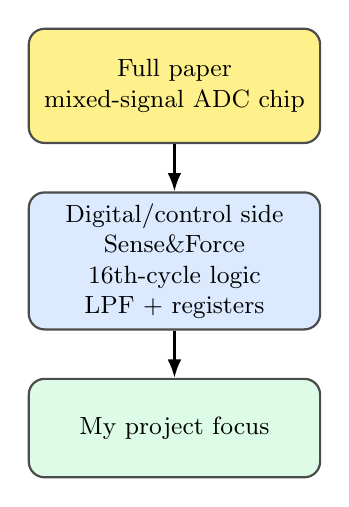
\begin{tikzpicture}[node distance=6mm]
        \node[block, fill=yellowbox, minimum width=3.7cm, minimum height=1.45cm] (chip) {Full paper\\mixed-signal ADC chip};
        \node[block, fill=navybox, below=of chip, minimum width=3.7cm, minimum height=1.7cm] (dig) {Digital/control side\\Sense\&Force\\16th-cycle logic\\LPF + registers};
        \node[block, fill=greenbox, below=of dig, minimum width=3.7cm, minimum height=1.25cm] (proj) {My project focus};
        \draw[line] (chip) -- (dig);
        \draw[line] (dig) -- (proj);
      \end{tikzpicture}
    \end{column}
  \end{columns}
\end{frame}

\begin{frame}{2. Architecture and Why Redundancy Matters}
  \begin{columns}[T]
    \begin{column}{0.55\textwidth}
      \small
      \begin{itemize}
        \item Final output is 13-bit, but the ADC uses \textbf{15 raw SAR cycles}.
        \item Two cycles are redundant, and an optional \textbf{16th cycle} is added only for calibration.
        \item Different 15-bit raw codes can map to the same final 13-bit result.
        \item That lets the controller compare two supposedly equal internal states and detect error from their sign difference.
      \end{itemize}
    \end{column}
    \begin{column}{0.45\textwidth}
      \centering
      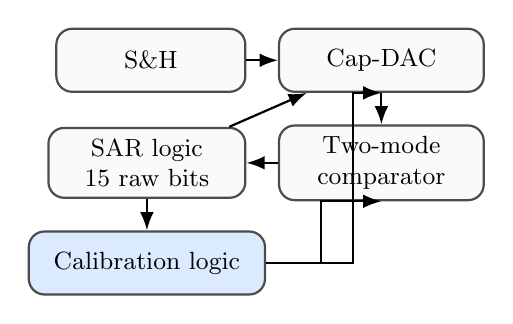
\begin{tikzpicture}[node distance=4mm]
        \node[block, fill=graybox, minimum width=2.4cm] (sh) {S\&H};
        \node[block, fill=graybox, right=of sh, minimum width=2.6cm] (dac) {Cap-DAC};
        \node[block, fill=graybox, below=of dac, minimum width=2.6cm] (comp) {Two-mode\\comparator};
        \node[block, fill=graybox, left=of comp, minimum width=2.5cm] (sar) {SAR logic\\15 raw bits};
        \node[block, fill=navybox, below=of sar, minimum width=3.0cm] (cal) {Calibration logic};
        \draw[line] (sh) -- (dac);
        \draw[line] (dac) -- (comp);
        \draw[line] (comp) -- (sar);
        \draw[line] (sar) -- (dac);
        \draw[line] (sar) -- (cal);
        \draw[line] (cal.east) -- ++(0.7,0) |- (comp.south);
        \draw[line] (cal.east) -- ++(1.1,0) |- (dac.south);
      \end{tikzpicture}

      \vspace{2mm}

      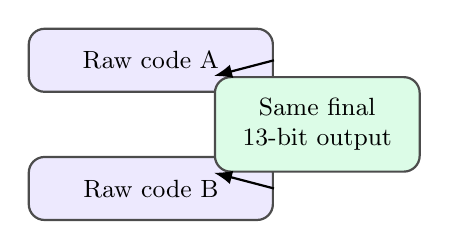
\begin{tikzpicture}[node distance=6mm]
        \node[block, fill=purplebox, minimum width=3.1cm] (a) {Raw code A};
        \node[block, fill=purplebox, below=8mm of a, minimum width=3.1cm] (b) {Raw code B};
        \node[block, fill=greenbox, right=8mm of $(a)!0.5!(b)$, minimum width=2.6cm, minimum height=1.2cm] (out) {Same final\\13-bit output};
        \draw[line] (a.east) -- (out.north west);
        \draw[line] (b.east) -- (out.south west);
      \end{tikzpicture}
    \end{column}
  \end{columns}
\end{frame}

\begin{frame}{3. Sign-Based Error Detection}
  \begin{columns}[T]
    \begin{column}{0.58\textwidth}
      \small
      \textbf{Key simplification:} the digital logic does \textbf{not} estimate exact error magnitude. It only decides whether correction should go \textbf{up} or \textbf{down}.

      \vspace{1mm}
      \begin{itemize}
        \item The system adds an optional \textbf{16th comparison cycle}.
        \item \textbf{Comparator offset detection:}
        \item compare \(D_{15}\) and \(D_{16}\) while switching comparator mode.
        \item \textbf{DAC mismatch detection:}
        \item detect a trigger code, then force the alternate redundant code \(A \leftrightarrow B\) during the 16th cycle.
        \item The sign of the change tells the controller whether the trim word must increase or decrease.
      \end{itemize}
    \end{column}
    \begin{column}{0.42\textwidth}
      \centering
      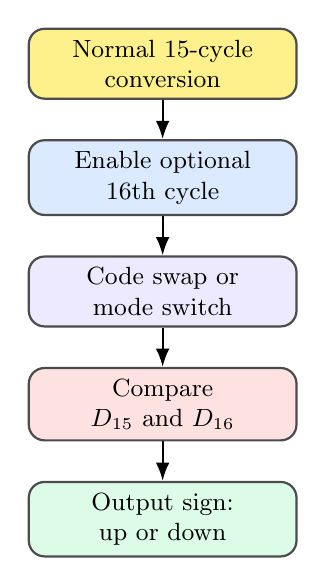
\begin{tikzpicture}[node distance=5mm]
        \node[block, fill=yellowbox, minimum width=3.4cm] (n1) {Normal 15-cycle\\conversion};
        \node[block, fill=navybox, below=of n1, minimum width=3.4cm] (n2) {Enable optional\\16th cycle};
        \node[block, fill=purplebox, below=of n2, minimum width=3.4cm] (n3) {Code swap or\\mode switch};
        \node[block, fill=pinkbox, below=of n3, minimum width=3.4cm] (n4) {Compare\\\(D_{15}\) and \(D_{16}\)};
        \node[block, fill=greenbox, below=of n4, minimum width=3.4cm] (n5) {Output sign:\\up or down};
        \draw[line] (n1) -- (n2);
        \draw[line] (n2) -- (n3);
        \draw[line] (n3) -- (n4);
        \draw[line] (n4) -- (n5);
      \end{tikzpicture}
    \end{column}
  \end{columns}
\end{frame}

\begin{frame}{4. Low-Power Sense\&Force Logic}
  \begin{columns}[T]
    \begin{column}{0.54\textwidth}
      \small
      \begin{itemize}
        \item Calibration only activates for \textbf{specific trigger patterns} in the 15-bit internal code.
        \item This happens only about \textbf{1.4\%} of the time.
        \item The paper uses custom \textbf{dynamic logic} instead of standard CMOS detection logic.
        \item Most of the time the detection slices stay reset/inactive, so they do not waste switching power.
        \item Functionally, this block is the \textbf{gatekeeper}: it senses the code and forces the correct 16th-cycle action.
      \end{itemize}
    \end{column}
    \begin{column}{0.46\textwidth}
      \centering
      \scriptsize
      \begin{tabular}{|l|c|c|}
        \hline
        Target & \(X\) trigger & \(Y\) \\
        \hline
        MSB   & 0111111 / 1000000 & 110 \\
        MSB-1 & 0011111 / 0100000 & 110 \\
        MSB-2 & 0101111 / 0110000 & 110 \\
        MSB-3 & 0110111 / 0111000 & 110 \\
        MSB-4 & 0111011 / 0111100 & 110 \\
        Comp. & 11000XX & 110 \\
        \hline
      \end{tabular}

      \vspace{4mm}

      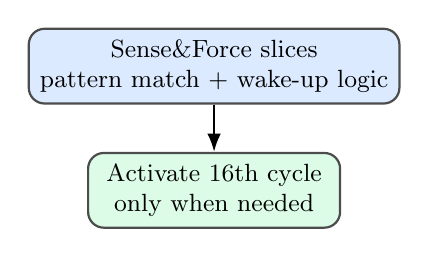
\begin{tikzpicture}[node distance=6mm]
        \node[block, fill=navybox, minimum width=3.7cm] (sense) {Sense\&Force slices\\pattern match + wake-up logic};
        \node[block, fill=greenbox, below=of sense, minimum width=3.2cm] (act) {Activate 16th cycle\\only when needed};
        \draw[line] (sense) -- (act);
      \end{tikzpicture}
    \end{column}
  \end{columns}
\end{frame}

\begin{frame}{5. Digital Feedback Loop: LPF, Registers, Reconstruction}
  \begin{columns}[T]
    \begin{column}{0.56\textwidth}
      \small
      \begin{itemize}
        \item There are \textbf{six} calibration paths:
        \item five DAC calibration paths + one comparator path.
        \item Each path has a \textbf{6-bit bidirectional counter} acting as a digital LPF.
        \item Random sign flips due to noise do not immediately update the trim value.
        \item Only when the counter hits its limit does it emit a step pulse to the calibration register.
        \item The ADC also produces a \textbf{15-bit raw code}; an \textbf{on-chip adder} converts that to the final 13-bit output.
      \end{itemize}
    \end{column}
    \begin{column}{0.44\textwidth}
      \centering
      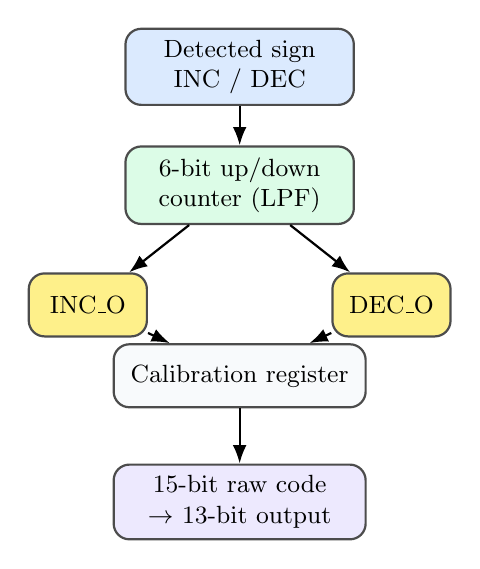
\begin{tikzpicture}[node distance=5mm]
        \node[block, fill=navybox, minimum width=2.9cm] (i) {Detected sign\\INC / DEC};
        \node[block, fill=greenbox, below=of i, minimum width=2.9cm] (c) {6-bit up/down\\counter (LPF)};
        \node[block, fill=yellowbox, below left=6mm and -3mm of c, minimum width=1.5cm] (u) {INC\_O};
        \node[block, fill=yellowbox, below right=6mm and -3mm of c, minimum width=1.5cm] (d) {DEC\_O};
        \node[block, fill=graybox, below=15mm of c, minimum width=3.2cm] (r) {Calibration register};
        \node[block, fill=purplebox, below=7mm of r, minimum width=3.2cm] (a) {15-bit raw code\\$\rightarrow$ 13-bit output};
        \draw[line] (i) -- (c);
        \draw[line] (c) -- (u);
        \draw[line] (c) -- (d);
        \draw[line] (u) -- (r);
        \draw[line] (d) -- (r);
        \draw[line] (r) -- (a);
      \end{tikzpicture}
    \end{column}
  \end{columns}
\end{frame}

\begin{frame}{6. Why This Works Well for an FPGA/HLS Project}
  \begin{columns}[T]
    \begin{column}{0.58\textwidth}
      \small
      \textbf{What maps directly to digital design}
      \begin{itemize}
        \item trigger-code detector
        \item 16th-cycle controller / FSM
        \item \(D_{15}\) vs \(D_{16}\) sign logic
        \item LPF counters
        \item calibration registers
        \item raw-to-final code adder
      \end{itemize}

      \textbf{What I would model, not physically build}
      \begin{itemize}
        \item DAC mismatch
        \item comparator offset/noise
        \item analog correction capacitors
      \end{itemize}
    \end{column}
    \begin{column}{0.42\textwidth}
      \centering
      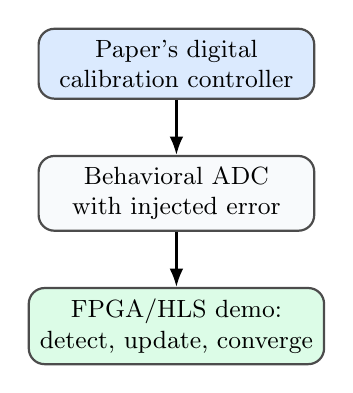
\begin{tikzpicture}[node distance=7mm]
        \node[block, fill=navybox, minimum width=3.5cm] (d) {Paper's digital\\calibration controller};
        \node[block, fill=graybox, below=of d, minimum width=3.5cm] (m) {Behavioral ADC\\with injected error};
        \node[block, fill=greenbox, below=of m, minimum width=3.5cm] (o) {FPGA/HLS demo:\\detect, update, converge};
        \draw[line] (d) -- (m);
        \draw[line] (m) -- (o);
      \end{tikzpicture}
    \end{column}
  \end{columns}
\end{frame}

\begin{frame}{7. Reported Results and Takeaways}
  \begin{columns}[T]
    \begin{column}{0.56\textwidth}
      \small
      \textbf{Measured results in the paper}
      \begin{itemize}
        \item 46 \(\mu\)W total power at 6.4 MS/s
        \item 64.1 dB SNDR at Nyquist
        \item 81.9 dB SFDR
        \item about 20 dB spur suppression from calibration
        \item convergence in about 400k cycles
      \end{itemize}

      \textbf{Main takeaway}
      \begin{itemize}
        \item The analog hardware applies the physical correction, but the \textbf{digital logic is the intelligence of the system}.
        \item It monitors behavior, decides the sign of the error, filters noise, and manages the feedback loop with very low complexity.
      \end{itemize}
    \end{column}
    \begin{column}{0.44\textwidth}
      \centering
      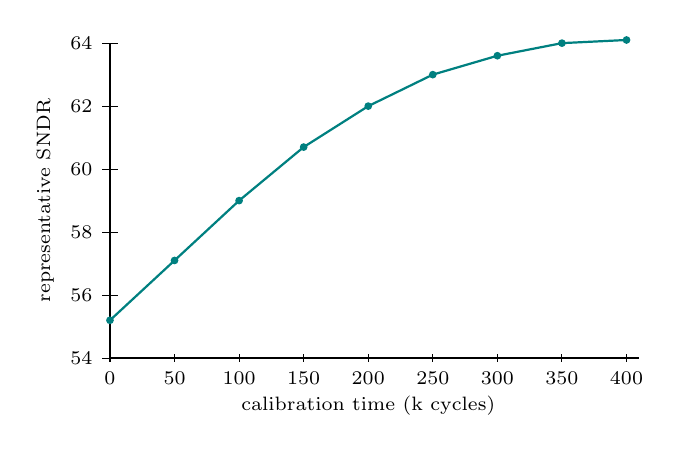
\begin{tikzpicture}[x=0.82cm,y=0.4cm]
        \draw[thick] (0,0) -- (0,10);
        \draw[thick] (0,0) -- (8.2,0);
        \foreach \y/\label in {0/54,2/56,4/58,6/60,8/62,10/64} {
          \draw (-0.12,\y) -- (0.12,\y);
          \node[left] at (-0.12,\y) {\scriptsize \label};
        }
        \foreach \x/\label in {0/0,1/50,2/100,3/150,4/200,5/250,6/300,7/350,8/400} {
          \draw (\x,-0.12) -- (\x,0.12);
          \node[below] at (\x,-0.12) {\scriptsize \label};
        }
        \node[below] at (4,-0.9) {\scriptsize calibration time (k cycles)};
        \node[rotate=90] at (-1.0,5) {\scriptsize representative SNDR};
        \draw[thick, teal] plot coordinates {(0,1.2) (1,3.1) (2,5.0) (3,6.7) (4,8.0) (5,9.0) (6,9.6) (7,10.0) (8,10.1)};
        \foreach \x/\y in {0/1.2,1/3.1,2/5.0,3/6.7,4/8.0,5/9.0,6/9.6,7/10.0,8/10.1} {
          \fill[teal] (\x,\y) circle (1.4pt);
        }
      \end{tikzpicture}
    \end{column}
  \end{columns}
\end{frame}

\end{document}
